\subsubsection{DHCP aktivieren}
\begin{lstlisting}
Router>en
Router#conf t
Router(config)#ip dhcp excluded-address 192.168.1.1 192.168.1.10
Router(config)#ip dhcp excluded-address 192.168.2.1 192.168.2.10
Router(config)#ip dhcp pool Users
Router(dhcp-config)#network 192.168.1.0 255.255.255.0
Router(dhcp-config)#default-router 192.168.1.254
Router(dhcp-config)#dns-server 192.168.1.254
Router(dhcp-config)#exit
Router(config)#ip dhcp pool Admins
Router(dhcp-config)#network 192.168.2.0 255.255.255.0
Router(dhcp-config)#default-router 192.168.2.254
Router(dhcp-config)#dns-server 192.168.2.254
Router(dhcp-config)#end
\end{lstlisting}
\paragraph{Resultate}
\begin{figure}[!htb]
    \centering
    \begin{subfigure}{\textwidth}
        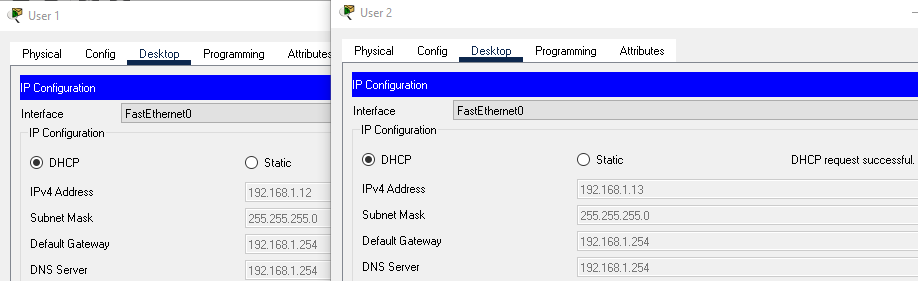
\includegraphics[width=\textwidth,height=.85\textwidth,keepaspectratio]{./img/users_dhcp.png}
        \caption{User PCs}
    \end{subfigure}
    \begin{subfigure}{\textwidth}
        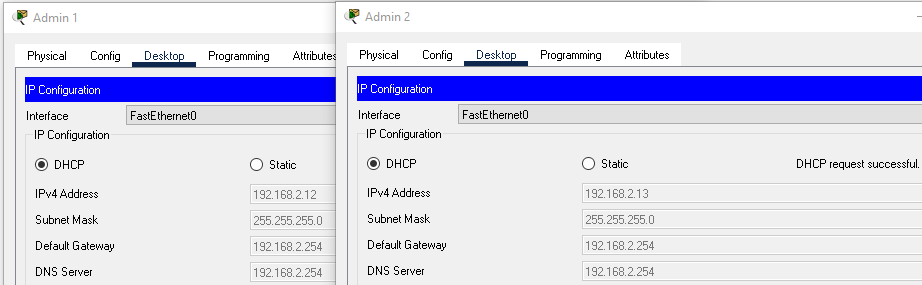
\includegraphics[width=\textwidth,height=.85\textwidth,keepaspectratio]{./img/admins_dhcp.png}
        \caption{Admin PCs}
    \end{subfigure}
    \caption{DHCP an den Endsystemen}
\end{figure}
\subsubsection{Frage 1}
\paragraph{Frage}
Woher weiß der Router, aus welchem Pool er die Adressen an die
anfragenden Clients (also PCs) zuweisen soll?
\paragraph{Antwort}
Bei der letzten Übung wurden die "dot1q encapsulation" beim Router aktiviert. Dadurch wurde jedem Subinterface eine bestimmte vlan-id zugewiesen. Jeder Subinterface weiß dadurch welchen Geräten er welche Adresse zuweisen muss.